% !TEX root = ../main.tex

\chapter{Evaluation}
\label{chap:evaluation}

\section{Evaluation Design and Dataset Rationale}

This chapter evaluates whether the safety layer reliably detects maladaptive rewriting actions in controlled IRT-style examples. The evaluation focuses on the implemented critic pipeline, not on clinical treatment efficacy. In other words, the question is not whether the chatbot treats nightmares, but whether the safety layer detects and redirects rewriting actions that the ontology defines as maladaptive.

The primary evaluation uses synthetic benchmark scenarios. This was practical because real IRT rescripting transcripts were not available at the required scale, and useful because synthetic cases allowed controlled coverage of the ontology categories. Real IRT transcript collection would also raise substantial privacy and ethics constraints. Synthetic data made it possible to cover all ontology categories, include safety-relevant maladaptive patterns, and construct targeted boundary cases with known expected labels. Because the same labelled benchmark was used across all runs, it also allowed direct comparison between classifier and pipeline variants. At the same time, synthetic benchmarks are only a controlled proxy. They can test whether the system applies the formalized safety categories under known conditions, but they cannot establish real-world clinical safety.

\subsection{Evaluation Goals}

The evaluation has four goals. First, it tests whether the critic distinguishes adaptive and maladaptive rewriting actions at the binary safety level. This is the most important operational question for the safety layer: maladaptive actions should not pass through as safe.

Second, it tests whether the critic assigns the intended ontology category. This is a stricter task than binary safety detection. A prediction can be safe at the binary level while still selecting a different adaptive or neutral node than the benchmark label. For example, an environmental mastery action may be classified as behavioral mastery without creating a safety failure. Node-level performance therefore measures how precisely the critic applies the ontology, not only whether it avoids the most clinically important errors.

Third, the evaluation compares design choices in the safety layer. This includes the direct System 1 classifier, the structured-reasoning System 2 classifier, semantic consistency, and ablations of the segmentation and meta-filtering pipeline. These comparisons are used to ask whether added complexity improves the safety decision enough to justify its cost and failure modes.

Fourth, the evaluation examines uncertainty signals. The thesis compares token log-probability confidence with semantic consistency to test whether either signal helps identify less reliable classifications. This is especially important because the safety layer is intended as an auditable critic: it should not only return a label, but also expose when that label may be less stable.

\subsection{Rationale for Synthetic Benchmarking}

The benchmark is synthetic because the target task requires controlled coverage of clinically specific and safety-relevant rewriting patterns. Some categories, such as violent revenge or unchanged trauma replay, cannot be assumed to occur often enough in a small natural transcript sample for systematic evaluation. A naturalistic dataset would therefore need to be large, sensitive, and carefully annotated to cover all categories adequately.

Synthetic generation allowed the evaluation to start from predefined nightmare scenarios and create matched rewriting attempts for each ontology category. This gave the benchmark a balanced structure: adaptive mastery categories, maladaptive categories, neutral categories, mixed inputs, and meta-level conversation could all be represented deliberately. It also made it possible to construct examples that differ in safety-relevant ways while sharing the same nightmare context.

This design has limits. Generated cases may contain phrasing patterns that are more explicit than real client language. They may also overrepresent clean category boundaries, because the generation process knows the target label. For this reason, the benchmark is best interpreted as an end-to-end test of the safety critic under controlled conditions. It supports claims about category application, pipeline behavior, and uncertainty estimation, but not claims about clinical effectiveness or deployment readiness.

\subsection{Dataset Construction}

The main development benchmark contains 480 cases across ten nightmare scenarios. Each scenario provides a short nightmare context and a set of rewriting-stage user inputs. The contexts cover different threat structures, such as being chased, being trapped, being publicly humiliated, facing a threatening intruder, or being unable to move while danger approaches. Each user input is evaluated together with the scenario context, matching the way the safety critic is used during the chatbot's rewriting stage.

Each benchmark case contains a user input, an expected binary safety label where applicable, and an expected primary ontology node where applicable. The development set contains 420 scored cases with both safety and node labels, plus 60 boundary cases without expected labels. These unscored boundary cases are retained for qualitative analysis but excluded from the primary accuracy denominators. Among the 420 scored cases, 240 are expected to be safe and 180 are expected to be unsafe.

A concrete example of one benchmark scenario and representative labelled user turns is provided in \Cref{app:benchmark-example}.

The benchmark also includes multipart cases. These inputs combine more than one kind of material in a single user turn, such as a conversational aside plus a rewriting action, or an adaptive element plus a maladaptive element. Multipart cases are important because the critic is not only a classifier; it is a pipeline that segments, filters, classifies, aggregates, and synthesizes constraints. A whole-turn label would hide failures in these intermediate steps.

\todo{Expand this dataset-construction subsection with a more explicit account of how the synthetic data was generated from \texttt{experiments/generate\_dataset.py}: scenario theme selection, GPT-5.4 generation of nightmare contexts, category-targeted rewriting actions, neutral cases, multipart patterns, and prompt revisions after quality-control findings. Also mention that full generation prompts are available in the appendix or repository.}

\todo{Explain the deliberately planned boundary cases, not only that they existed. State that boundary cases were generated from predefined clinically important pairs: behavioral mastery vs. violent revenge (proportionality), avoidance vs. affect expression (passivity), emotional mastery vs. suppression (regulation vs. denial), narrative setting vs. trauma replay (description vs. unchanged replay), behavioral mastery vs. avoidance (active coping vs. escape), and behavioral mastery vs. interruption (action vs. ending the dream). Explain that these cases were kept out of primary accuracy denominators because the point was exploratory ambiguity analysis rather than fixed-label scoring.}

\subsection{Scenario and Category Coverage}

The development benchmark covers all ontology nodes used by the critic pipeline. The labelled portion contains cases for the five adaptive mastery nodes, the five maladaptive nodes, and the two neutral nodes. The unscored rows are used for boundary material where a strict node label would be less meaningful for the primary quantitative analysis.

The nightmare scenarios were selected to cover both clinically common dream themes and the specific contexts needed to test the ontology. The broader context library was guided by theme distributions reported in nightmare research, including attack, chase, falling, trapped or helpless situations, social threat, loss, and supernatural content \parencite{schredl2018nightmare}. At the same time, exact prevalence matching was not the goal. Some themes were included or weighted because they are especially useful for evaluating particular safety distinctions: attack scenarios for violent revenge versus behavioral mastery, trapped or chase scenarios for avoidance and interruption, social and loss scenarios for suppression and emotional mastery, supernatural scenarios for mythical mastery, and trauma-replay scenarios for unchanged repetition.

\Cref{tab:benchmark-datasets} summarizes the main benchmark material. The development set is the primary source for component-level variant comparisons because all classifier, consistency, and ablation conditions were run on it. A separate held-out test set was generated to assess generalization of the selected critic configuration. It contains 315 cases across seven scenarios, of which 273 have expected node labels. In the test set, clean and multipart cases provide the main safety metrics. Boundary cases are reported separately because they do not have fixed expected labels; they are used to explore classifier behavior on ambiguous inputs rather than to compute primary accuracy. They also follow repeated templates across scenarios, which further limits their ecological validity.

\begin{table}
  \centering
  \caption{Benchmark datasets used for evaluation.}
  \label{tab:benchmark-datasets}
  \renewcommand{\arraystretch}{1.25}
  \small
  \setlength{\tabcolsep}{4pt}
  \begin{tabular}{>{\raggedright\arraybackslash}p{0.24\linewidth}>{\raggedright\arraybackslash}p{0.20\linewidth}>{\raggedright\arraybackslash}p{0.10\linewidth}>{\raggedright\arraybackslash}p{0.34\linewidth}}
    \toprule
    Dataset & Scenario source & Cases & Role in the thesis \\
    \midrule
    Development benchmark & 10 scenarios & 480 & Primary component-level benchmark for classifier, consistency, and ablation comparisons; 420 scored cases and 60 unscored boundary cases. \\
    Held-out test set & 7 scenarios & 315 & Generalization check for the selected critic configuration; clean and multipart cases provide the main test-set metrics, with boundary cases reported separately. \\
    Composite maladaptive slice & 5 reused development scenarios & 35 & Supplementary stress test for inputs that combine two maladaptive patterns in one rewriting turn. \\
    \bottomrule
  \end{tabular}
\end{table}

\subsection{Human / Expert Annotation Material}

The ontology itself was reviewed by Dr. Annika Gieselmann, as described in \Cref{sec:clinical-rationale-boundaries}. For the benchmark material, the labels were generated with the dataset and then partially reviewed by the author to check whether the expected safety labels and ontology nodes matched the clinical definitions used in this thesis. This review covered all available boundary cases, all affect-expression cases, all violent-revenge cases, and a stratified spot check across the remaining nodes.

Because the benchmark labels were generated together with the cases, they were not
treated as automatically correct. Several quality-control passes were used to identify
cases where the generated action did not clearly match the intended label or where the
phrasing introduced dataset artifacts. Earlier generation passes exposed
meta-narration and affect-expression problems, which led to prompt revisions and
regenerated benchmark material. In the held-out test material, one truncated nightmare
suite was excluded, and templated boundary cases were separated from the primary scored
analysis. The resulting labels should therefore be understood as synthetic benchmark
labels with targeted author review, not as independent expert ground truth.

This review should not be interpreted as independent inter-rater reliability. It was an internal label-quality check, not a blinded expert annotation study. Its main purpose was to catch obvious generation errors before using the data for system evaluation. Expert-facing material for system-level comparison is discussed separately in \Cref{sec:system-level-expert-evaluation}.

\todo{Work in dataset-quality caveat: dev-set spot check found 33/36 agreement, with all 3 disagreements concentrated in AFFECT\_EXPRESSION cases that were better interpreted as unsafe TRAUMA\_REPLAY. Explain that this may make some development-set false positives clinically plausible label-noise rather than classifier errors. Also state that the held-out test set mitigates this because all valid AFFECT\_EXPRESSION cases were manually reviewed; remaining test-set concern is mainly ecological validity / overlap with EMOTIONAL\_MASTERY, not binary safety disagreement.}

\todo{Obtain independent expert annotations for the held-out test set from Katharina Lüth and Dr. Annika Gieselmann; use them for targeted expert validation and inter-rater agreement where possible.}

\todo{Include a focused expert spot check of violent-revenge cases, especially boundary cases where proportionate self-protection and maladaptive retaliation are difficult to separate from text alone.}

\begin{figure}
  \centering
  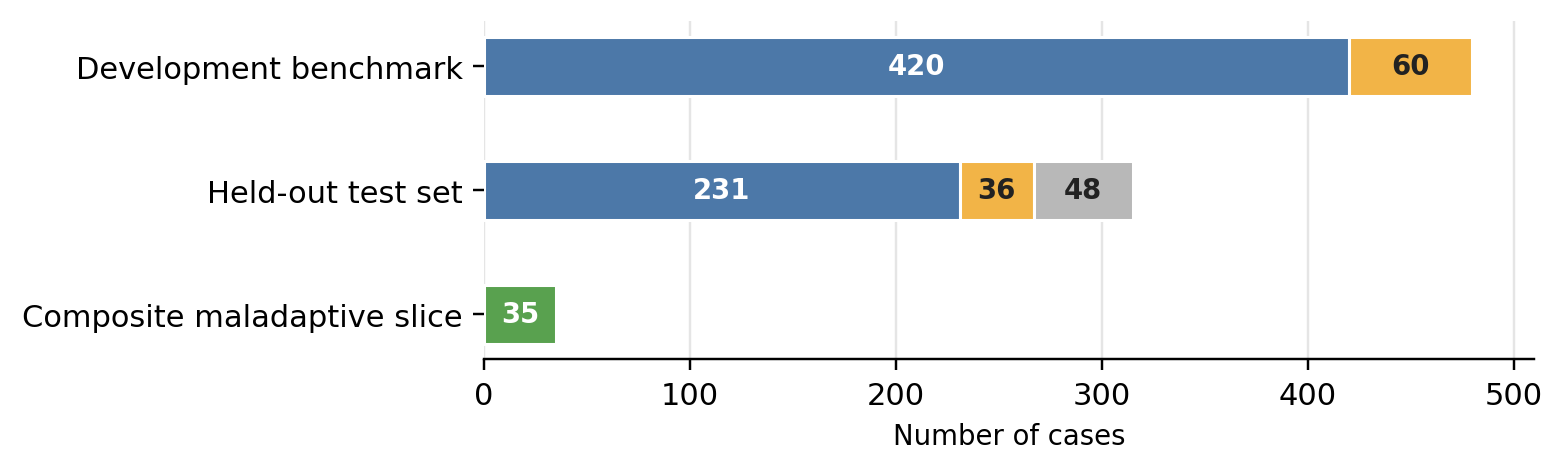
\includegraphics[width=0.92\linewidth]{../figures/evaluation_materials_overview.png}
  \caption{Evaluation material by scoring status. Blue segments contain cases used for scored development or test-set metrics, yellow segments contain exploratory boundary cases, grey marks the excluded truncated buried-alive suite, and green marks the supplementary composite-maladaptive stress test.}
  \label{fig:dataset-composition}
\end{figure}

\section{Experimental Conditions and Metrics}

The experiments compare classifier variants, uncertainty methods, and pipeline variants while keeping the ontology fixed. This is important because the thesis evaluates the safety layer as an implemented system, not only as a set of category definitions. All component-level conditions use the same benchmark labels and the same top-level scoring logic: the critic receives a user input and nightmare context, returns a structured safety result, and that result is compared with the case-level benchmark label.

\subsection{Classifier Variants: System 1 and System 2}

Two classifier variants are evaluated. System 1 is the direct classifier: it receives the category definitions and decision rules and returns a single semantic code, which is then mapped to an ontology node. System 2 uses the same category definitions and decision rules, but returns a structured rationale before giving the final code.

The comparison tests a simple question: does explicit reasoning improve ontology classification enough to justify the additional generation length, parsing complexity, latency, and weaker single-token confidence signal? The rest of the critic pipeline is held constant when comparing the two classifiers, so differences in performance can be attributed mainly to the classifier output format and reasoning step rather than to different safety categories.

\subsection{Pipeline Variants and Ablations}

The main pipeline condition is the structured safety critic described in \Cref{sec:safety-critic-pipeline}: LLM-based segmentation, meta-statement filtering, segment-level classification, aggregation, severity triage, and constraint synthesis. This full pipeline is the condition used for the main System 1 and System 2 results.

Ablation experiments are used to test whether the pipeline components contribute in the expected way. The no-segmentation condition forces the whole user turn into a single action segment. The meta-filtering ablation keeps segments labelled as \texttt{META} instead of removing them before dream-content classification. A naive-segmentation condition replaces the LLM segmenter with sentence splitting. A stage-merge condition combines segmentation and classification into one model call. These ablations are not alternative clinical systems proposed for deployment; they are diagnostic conditions used to understand which parts of the pipeline matter.

The ablation analysis is reported separately because it asks a different question from the main classifier comparison. The main comparison asks which classifier variant works best inside the full critic. The ablations ask how much the surrounding pipeline shapes the final safety decision.

\subsection{Uncertainty Methods: Log-Probabilities and Semantic Consistency}

Two uncertainty methods are evaluated. The first is token log-probability confidence from a single classifier call. For System 1, this is the length-normalized probability of the generated classification code. This value is available at no extra inference cost when the provider returns log probabilities.

The second method is semantic consistency. In this condition, the classifier is run multiple times on the same segment using stochastic sampling, and the resulting labels are aggregated by majority vote. The agreement ratio is used as an uncertainty signal: high agreement means repeated runs converged on the same category, while lower agreement indicates that the classification was less stable.

Semantic consistency is more expensive because it requires repeated classifier calls. It also measures only the stability of the classification step. If the segmenter removes or mislabels relevant content before classification, repeated classification cannot recover it. For this reason, uncertainty results are interpreted as classification-level signals rather than as guarantees about the whole pipeline.

\subsection{Evaluation Metrics}

The primary metric is binary safety accuracy. It measures whether the critic's final safety verdict matches the expected safe or unsafe label. Because the safety layer is designed to catch maladaptive rewriting actions, unsafe recall is reported as a key metric: it measures the proportion of expected unsafe cases that the critic correctly flags as unsafe. Unsafe precision and unsafe F1 are also useful for describing the false-alarm trade-off, but unsafe recall carries the strongest safety interpretation.

The second main metric is strict primary-node accuracy. The benchmark labels each scored case with one expected ontology node. The critic may internally classify multiple segments, but the quantitative node metric compares only the final triaged \texttt{result.node\_id} with the case's \texttt{expected\_node}. For multipart cases, this expected node is the node that should dominate after triage, not a complete list of all valid segment labels.

This distinction is important. The benchmark does not contain gold segment boundaries or gold labels for every internal segment. Segment predictions are logged and used for qualitative error analysis, but the reported node accuracy is a case-level primary-node metric. A node error therefore does not always mean that the critic misunderstood every part of the input. It means that the final node selected for the case did not match the benchmark's expected primary node.

Segmentation is therefore not evaluated as a separate gold-standard task. Creating such a benchmark would require manual segment-boundary annotation, segment-level node labels, and agreement checks for each segment. This would be a substantial additional annotation study and would introduce its own boundary decisions. Instead, segmentation is evaluated indirectly through its effect on the final case-level safety verdict and primary-node prediction.

\begin{table}
  \centering
  \caption{Main evaluation metrics.}
  \label{tab:evaluation-metrics}
  \renewcommand{\arraystretch}{1.18}
  \begin{tabular}{p{0.28\linewidth}p{0.58\linewidth}}
    \toprule
    Metric & Interpretation \\
    \midrule
    Safety accuracy & Proportion of scored cases where the final safe/unsafe verdict matches the benchmark label. \\
    Unsafe recall & Proportion of expected unsafe cases correctly flagged as unsafe. This is the main safety-sensitive metric. \\
    Unsafe precision & Proportion of predicted unsafe cases that are truly unsafe, indicating the false-alarm burden. \\
    Primary-node accuracy & Proportion of cases where the final triaged ontology node matches the expected case-level node. \\
    Agreement ratio & Proportion of semantic-consistency runs supporting the majority label. Used as an uncertainty signal. \\
    \bottomrule
  \end{tabular}
\end{table}

\subsection{Reproducibility and Implementation Details}

The benchmark runner is implemented in \texttt{experiments/run\_benchmark.py}. It loads a JSON benchmark dataset, runs the safety critic on each case, and writes a CSV file containing the expected labels, predicted labels, confidence values, severity labels, extracted contexts, and serialized segment results. The main development-set runs use \texttt{data/benchmarks/dev\_dataset.json}; the corresponding result files are stored under \texttt{data/benchmarks/}.

The reported benchmark configuration uses deterministic baselines for both classifier variants. Both System 1 and System 2 use Mistral Small 3.2 via Scaleway with temperature 0. The segmentation step uses the smaller Mistral Nemo model via Scaleway with temperature 0. This separates the lightweight preprocessing step from the ontology classification step while keeping both stages on the same provider backend.

Mistral Small was chosen for classification because it supports the required log-probability outputs, is lightweight enough for repeated benchmark runs, and keeps the System 1 and System 2 comparison controlled by using the same underlying model. The use of Mistral-family models also matches the baseline chatbot system, which was built around European model providers for GDPR-oriented data-hosting reasons. Mistral Nemo was used for segmentation because the task is narrower and mainly requires deterministic, low-cost structured extraction. Semantic consistency uses five stochastic classification runs with temperature 0.7. Although the models were accessed through Scaleway rather than Mistral's own API, this value was chosen to introduce meaningful variation between repeated runs while staying within Mistral's public temperature guidance of 0.0 to 0.7 \parencite{mistralApiDocs}. This separates the deterministic point estimate from the repeated-sampling uncertainty condition. Transient API failures are handled with retry logic in the agent wrapper, which is important for long benchmark runs.

\Cref{tab:experimental-conditions} summarizes the main safety-critic benchmark conditions. The exact prompts are included in the appendix, and the CSV outputs provide the audit trail for each individual benchmark case.

\begin{table}
  \centering
  \caption{Main experimental conditions for the safety-critic benchmark.}
  \label{tab:experimental-conditions}
  \small
  \setlength{\tabcolsep}{4pt}
  \renewcommand{\arraystretch}{1.12}
  \begin{tabular}{>{\raggedright\arraybackslash}p{0.20\linewidth}>{\raggedright\arraybackslash}p{0.23\linewidth}>{\raggedright\arraybackslash}p{0.45\linewidth}}
    \toprule
    Condition & Classifier & Purpose \\
    \midrule
    S1 baseline & Direct code output & Primary direct-classification reference condition. \\
    \addlinespace[0.35em]
    S1 consistency & Direct code output, repeated & Tests whether semantic consistency improves or calibrates System 1. \\
    \addlinespace[0.35em]
    S2 baseline & Structured reasoning & Tests whether rationale-first classification improves ontology mapping. \\
    \addlinespace[0.35em]
    S2 consistency & Structured reasoning, repeated & Tests whether repeated reasoning exposes uncertainty in System 2. \\
    \addlinespace[0.35em]
    Ablations & S1 unless stated otherwise & Tests the contribution of segmentation, meta filtering, naive segmentation, and stage-merged processing. \\
    \bottomrule
  \end{tabular}
\end{table}

\begin{figure}
  \centering
  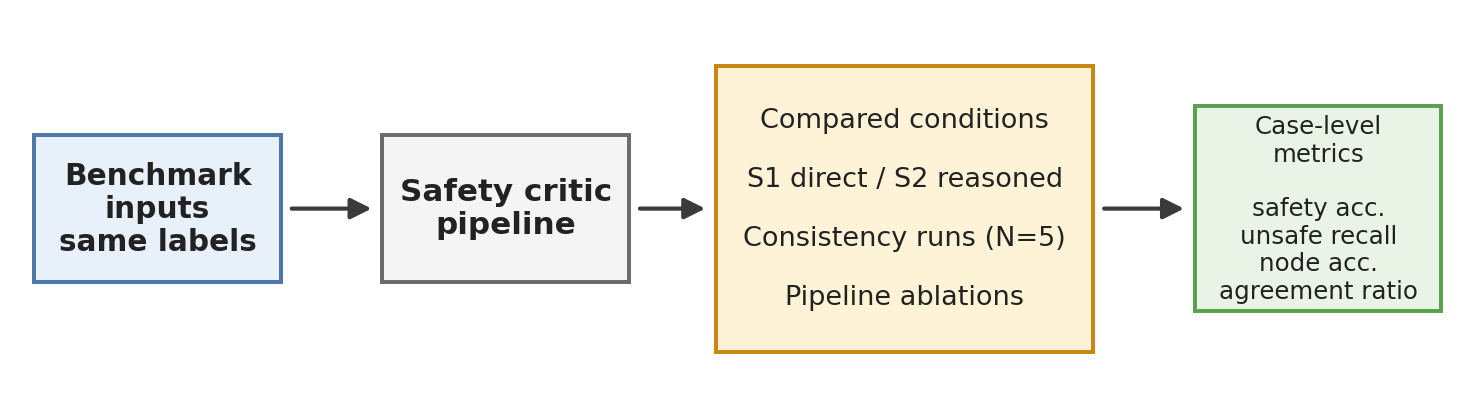
\includegraphics[width=0.98\linewidth]{../figures/experimental_design_overview.png}
  \caption{Safety-critic experimental design. The same labelled benchmark material is passed through the safety critic under classifier-variant, semantic-consistency, and ablation conditions, and all conditions are evaluated with the same case-level metrics.}
  \label{fig:experimental-design}
\end{figure}

\section{Safety Critic Classification Results}

The main safety-critic benchmark was run on the 480-case development set described above. The 420 scored cases are used for the quantitative metrics in this section; the 60 unscored boundary cases are excluded from the accuracy denominators. The reported runs use deterministic baseline settings: the segmenter runs through the direct Scaleway Mistral Nemo backend at temperature 0, the baseline classifiers run at temperature 0, and semantic consistency uses five stochastic classifier calls at temperature 0.7 after segmentation.

The headline result is that all four main configurations perform strongly on binary safety detection. Differences between conditions are therefore small in absolute terms, but they matter because the remaining errors have different safety implications. S2 with semantic consistency achieves the highest overall safety accuracy, mainly by reducing false alarms on safe cases. However, it also misses more unsafe cases than the other three configurations. For this reason, it should be interpreted as a precision--recall trade-off rather than as a simple improvement over the direct classifier.

\subsection{Overall Safety Classification Performance}

The overall safety results are shown in \Cref{tab:component-safety-results}. System 1 baseline correctly classified 411 of the 420 scored cases, corresponding to 97.86\% safety accuracy. It flagged 179 of the 180 unsafe cases, giving an unsafe recall of 99.44\%. Its remaining safety errors consisted of eight false alarms and one missed unsafe case.

System 2 baseline produced a very similar result. It also detected 179 of 180 unsafe cases, but reduced false alarms from eight to seven, raising safety accuracy slightly to 98.10\%. In this benchmark, structured reasoning matched the direct classifier on unsafe recall while producing one fewer false alarm. The gain is small, but it shows that the reasoning variant can reduce some false alarms without changing the main safety-sensitive metric in the single-run condition.

The strongest overall accuracy was obtained by System 2 with semantic consistency. This condition correctly classified 415 of 420 scored cases, or 98.81\%. The improvement came from a large reduction in false alarms: only two safe cases were incorrectly flagged as unsafe. The trade-off is that unsafe recall dropped to 177 of 180 cases, or 98.33\%. In a safety layer for IRT rescripting, this trade-off must be stated explicitly. A lower false-alarm rate can improve the user experience, but missed maladaptive rewriting actions carry the greater safety concern.

\begin{table}
  \centering
  \caption{Safety-critic classification results on the scored development benchmark.}
  \label{tab:component-safety-results}
  \small
  \setlength{\tabcolsep}{4pt}
  \renewcommand{\arraystretch}{1.35}
  \begin{tabular}{p{0.23\linewidth}p{0.18\linewidth}p{0.18\linewidth}p{0.14\linewidth}p{0.14\linewidth}}
    \toprule
    Condition & Safety accuracy & Unsafe recall & False alarms & Missed unsafe \\
    \midrule
    S1 baseline & 97.86\%\newline (411/420) & 99.44\%\newline (179/180) & 8 & 1 \\
    \addlinespace[0.25em]
    S1 consistency & 97.86\%\newline (411/420) & 99.44\%\newline (179/180) & 8 & 1 \\
    \addlinespace[0.25em]
    S2 baseline & 98.10\%\newline (412/420) & 99.44\%\newline (179/180) & 7 & 1 \\
    \addlinespace[0.25em]
    S2 consistency & \textbf{98.81\%}\newline (415/420) & 98.33\%\newline (177/180) & \textbf{2} & 3 \\
    \bottomrule
  \end{tabular}
\end{table}

\subsection{Node-Level Classification Performance}

Primary-node accuracy is lower than binary safety accuracy because it asks a stricter question. A case is counted as correct only when the final triaged ontology node matches the benchmark's expected primary node. Safe categories can therefore be confused with one another without producing a safety error. For example, an affect-expression case may be classified as emotional mastery, or a mythical mastery case may be classified as environmental mastery. These are ontology-level errors, but they usually do not mean that a maladaptive rewriting action passed through as safe.

\Cref{tab:component-node-results} reports strict primary-node accuracy over all 420 scored cases with expected nodes. This includes cases where the final pipeline output was \texttt{META\_ONLY}. Such cases are kept in the denominator because the metric evaluates the complete critic pipeline, not only the classifier after successful preprocessing. If a labelled case expects \texttt{NARRATIVE\_SETTING} but the pipeline filters the input as meta-conversation, that is a primary-node error in the implemented system.

System 1 baseline reached 78.10\% primary-node accuracy. System 2 baseline improved this to 79.05\%, and System 2 with semantic consistency reached 80.00\%. The modest gap between safety accuracy and node accuracy is expected in this task. The safety layer's most important job is to distinguish adaptive or neutral rewriting from maladaptive rewriting. Exact placement among neighboring safe categories is useful for auditability and response shaping, but less safety-critical than the binary unsafe decision.

\begin{table}
  \centering
  \caption{Strict primary-node accuracy on the scored development benchmark.}
  \label{tab:component-node-results}
  \small
  \setlength{\tabcolsep}{5pt}
  \renewcommand{\arraystretch}{1.12}
  \begin{tabular}{p{0.27\linewidth}p{0.22\linewidth}p{0.27\linewidth}p{0.14\linewidth}}
    \toprule
    Condition & Node accuracy & Unsafe-category node accuracy range & \texttt{META\_ONLY} outputs \\
    \midrule
    S1 baseline & 78.10\% (328/420) & 90.0--100.0\% & 4 \\
    S1 consistency & 78.10\% (328/420) & 90.0--100.0\% & 3 \\
    S2 baseline & 79.05\% (332/420) & 90.3--100.0\% & 3 \\
    S2 consistency & \textbf{80.00\%} (336/420) & 90.3--100.0\% & 3 \\
    \bottomrule
  \end{tabular}
\end{table}

The weakest node-level results occur mostly in safe or neutral categories. Affect expression is often classified as emotional mastery, because both involve emotional language and both are safe at the binary level. Mythical mastery is often confused with environmental mastery or behavioral mastery, especially when an imaginative change also alters the scene or involves active agency. These errors reduce primary-node accuracy but usually do not undermine the main safety function.

\todo{Add a short sensitivity analysis for the \texttt{AFFECT\_EXPRESSION} / \texttt{EMOTIONAL\_MASTERY} boundary. The current affect-expression generation prompt requires an emotional shift, which makes many cases read like emotional mastery rather than mere neutral affect expression. Admit this as an ontology/prompt-design limitation: affect expression is useful as a neutral segment label, but weak as a standalone primary rescripting category because real IRT clients usually express feelings together with an adaptive or maladaptive action. Report collapse numbers: if \texttt{AFFECT\_EXPRESSION} and \texttt{EMOTIONAL\_MASTERY} are merged for scoring, node accuracy rises from 328/420 (78.1\%) to 345/420 (82.1\%) for S1 consistency, from 336/420 (80.0\%) to 361/420 (86.0\%) for S2 consistency, and from 220/273 (80.6\%) to 230/273 (84.2\%) on the post-fix held-out test CSV. Emphasize that this mainly affects strict node accuracy, not the binary safety conclusion.}

The maladaptive categories are more stable. In the S2 consistency condition, \texttt{AVOIDANCE} and \texttt{INTERRUPTION} are classified with 100.0\% and 97.8\% node accuracy respectively, \texttt{SUPPRESSION} with 96.7\%, \texttt{TRAUMA\_REPLAY} with 93.3\%, and \texttt{VIOLENT\_REVENGE} with 90.3\%. The remaining maladaptive errors are therefore concentrated in a small number of boundary cases, discussed further in the failure analysis.

\subsection{System 1 vs. System 2 Comparison}

The comparison between System 1 and System 2 does not show a simple dominance pattern. System 2 baseline slightly improves both safety accuracy and primary-node accuracy relative to System 1 baseline while preserving the same unsafe recall. This suggests that the structured reasoning format can help in some ambiguous cases, especially by reducing false alarms.

At the same time, the gain is small. The difference between System 1 baseline and System 2 baseline is one additional correctly classified safety case and four additional correct primary-node predictions. This is not enough to justify treating System 2 as categorically better. System 2 also has practical disadvantages: it produces longer outputs, is slower, requires JSON parsing, and gives a less direct token-level confidence signal because the final label is generated after the model has already produced its rationale.

The most useful interpretation is therefore conservative. System 1 remains attractive as the primary classifier because it is simple, fast, and achieves very high unsafe recall. System 2 can reduce some false alarms, but its added reasoning step does not eliminate errors and does not clearly justify replacing the direct classifier in the main pipeline.

\subsection{Effect of Semantic Consistency}

Semantic consistency had different effects for the two classifier variants. For System 1, it did not change the headline safety or node metrics: both the baseline and consistency conditions achieved 411/420 safety accuracy and 328/420 node accuracy. In this benchmark, repeated sampling therefore did not add measurable classification benefit to the direct classifier.

For System 2, semantic consistency improved overall safety accuracy from 98.10\% to 98.81\% and node accuracy from 79.05\% to 80.00\%. The main benefit was fewer false alarms: S2 consistency reduced false alarms from seven to two. However, it also increased missed unsafe cases from one to three. This makes semantic consistency useful, but not unconditionally safer. It improves the system's ability to avoid over-flagging safe content, while slightly weakening the main safety-sensitive metric.

These results suggest a limited role for semantic consistency. It reduced false alarms for System 2, but it did not guarantee safer decisions overall, because the same condition also produced more missed unsafe cases. The limitation is also practical: with \(N=5\), each classified segment requires five stochastic classifier calls instead of one, increasing both inference cost and latency. Semantic consistency should therefore not be treated as a default replacement for single-run classification. Its more plausible role is as a stability signal for selected cases, while the cost, temperature setting, and decision rule for using this signal require further evaluation.

\section{Ablation and Pipeline Analysis}

The ablation experiments examine how much the surrounding critic pipeline shapes the
final safety decision. They are diagnostic rather than intended to identify a new
best-performing system variant. All ablations in this section use the System 1 classifier
without semantic consistency, so the results describe the direct-classification pipeline
only. The goal is therefore to understand which preprocessing choices affect classification
performance, not to evaluate every part of the safety layer separately.

The main question is how preprocessing and input structuring affect the case-level
safety verdict and the final primary-node prediction. This is important because the
critic is not a single classifier call. The full pipeline first segments the user turn,
filters meta-conversational material, classifies remaining dream-relevant segments, and
then aggregates the result. For this reason, the ablation results cannot be summarized
by a single metric: one variant may reduce false alarms, another may improve
primary-node selection, and another may preserve unsafe recall. For a safety layer,
these trade-offs must be interpreted separately.

The full S1 pipeline is the reference condition. It uses LLM-based segmentation, filters
\texttt{META} segments, classifies each remaining segment separately, and then applies
the usual aggregation and triage rules. The stage-merge condition replaces the separate
segmentation and classification calls with one model call that returns labelled
segments directly, including a \texttt{META} code for conversational content. The
no-segmentation condition passes the whole user turn to the classifier as a single
action segment. The META-filtering-off condition keeps the LLM segmenter but does not
remove \texttt{META} segments before classification; these segments are therefore
forced through the same 12-label classifier as dream-relevant content. The
naive-splitter condition replaces the LLM segmenter with simple sentence splitting.
Because this splitter does not assign \texttt{META} labels, all resulting segments are
passed to the classifier as action segments.

The conditions are not all interpreted against the full pipeline alone. Some comparisons
hold explicit \texttt{META} filtering off in both conditions, so that the effect of
segmentation can be examined without also changing the \texttt{META}-filtering step.
\Cref{tab:ablation-condition-interpretation} summarizes the intended pairwise
comparisons.

\begin{table}[!htbp]
  \centering
  \caption{Intended pairwise comparisons for the S1 ablation conditions.}
  \label{tab:ablation-condition-interpretation}
  \scriptsize
  \setlength{\tabcolsep}{3pt}
  \renewcommand{\arraystretch}{1.12}
  \begin{tabular}{@{}>{\raggedright\arraybackslash}p{0.24\linewidth}>{\raggedright\arraybackslash}p{0.30\linewidth}>{\raggedright\arraybackslash}p{0.38\linewidth}@{}}
    \toprule
    Comparison & Question & What is held constant \\
    \midrule
    Full S1 vs. META filtering off & What does \texttt{META} filtering contribute? & Same LLM segmentation, S1 classifier, and triage; only the filter changes. \\
    \addlinespace[0.2em]
    META filtering off vs. no segmentation & Does any segmentation help without explicit \texttt{META} filtering? & Explicit \texttt{META} filtering is absent in both; segmented input is compared with whole-turn input. \\
    \addlinespace[0.2em]
    META filtering off vs. naive splitter & Does LLM segmentation help beyond sentence splitting? & No explicit \texttt{META} filtering in either condition; semantic segments are compared with sentence chunks. \\
    \addlinespace[0.2em]
    Full S1 vs. stage-merge & Does two-stage processing help compared with one merged call? & Both can represent \texttt{META} content and use the same post-hoc triage logic. \\
    \bottomrule
  \end{tabular}
\end{table}

\subsection{Contribution of Pipeline Components}

The main ablation results are shown in \Cref{tab:ablation-main-results}. The full
System 1 pipeline reaches 97.86\% safety accuracy and detects 179 of 180 unsafe cases.
This is the highest unsafe recall among the main pipeline variants, tied only with the
META-filtering-off condition. Its errors are mostly false alarms: eight safe cases are
flagged as unsafe, while one unsafe case is missed.

The stage-merge condition combines segmentation and classification into one model call
and then applies the same symbolic triage logic after parsing the model output. It
achieves higher aggregate safety accuracy than the full pipeline, 98.33\% instead of
97.86\%, and substantially higher primary-node accuracy, 86.90\% instead of 78.10\%.
However, the gain comes with lower unsafe recall: it misses three unsafe cases rather
than one. This makes the result useful but not a simple replacement for the full
pipeline. It suggests that stage merging can improve primary-node accuracy, but it also
slightly reduces unsafe recall.

The no-segmentation condition forces the entire user turn into one action segment. If it
is compared directly with the full pipeline, it improves aggregate safety accuracy to
98.33\%, mainly because it produces no false alarms. Its closer diagnostic comparison,
however, is the META-filtering-off condition, because neither condition has explicit
\texttt{META} filtering. Read this way, no-segmentation avoids the false alarms that
occur when unfiltered \texttt{META} segments are classified as separate dream actions:
the classifier has to settle on one label for the whole turn instead. That same
single-label behavior also introduces a different risk. Several excessive-violence cases
are classified as adaptive mastery, suggesting that the active, agentic part of the
rewrite can dominate the violent-revenge signal. This is the clearest example of why
aggregate accuracy is not sufficient for this task.

The naive splitter is included as a simple sentence-boundary baseline. Its results are
closest to the no-segmentation condition: it recovers one additional unsafe case, but it
also introduces nine false alarms. Compared with the META-filtering-off condition, it
has fewer false alarms mainly because it does not semantically isolate conversational
fragments as separate classifier inputs. In this dataset, those fragments often remain
attached to an action sentence, so the classifier tends to settle on the action label
instead of assigning a maladaptive label to the conversational aside. This should not be
read as better handling of conversational content: the splitter can separate clean
two-sentence inputs, but the multipart inputs in this benchmark are often contained in a
single sentence, so sentence boundaries miss the structure that the LLM segmenter is
meant to recover.

\begin{table}
  \centering
  \caption{S1 ablation results on the scored development benchmark.}
  \label{tab:ablation-main-results}
  \footnotesize
  \setlength{\tabcolsep}{3pt}
  \renewcommand{\arraystretch}{1.25}
  \begin{tabular}{@{}>{\raggedright\arraybackslash}p{0.22\linewidth}>{\centering\arraybackslash}p{0.17\linewidth}>{\centering\arraybackslash}p{0.17\linewidth}>{\centering\arraybackslash}p{0.17\linewidth}>{\centering\arraybackslash}p{0.18\linewidth}@{}}
    \toprule
    Condition & \shortstack{Safety\\acc.} & \shortstack{Unsafe\\recall} & \shortstack{Primary node\\acc.} & \shortstack{False alarms /\\missed unsafe} \\
    \midrule
    Full S1 pipeline & 97.86\%\newline (411/420) & 99.44\%\newline (179/180) & 78.10\%\newline (328/420) & 8\,/\,1 \\
    \addlinespace[0.35em]
    Stage-merge & 98.33\%\newline (413/420) & 98.33\%\newline (177/180) & 86.90\%\newline (365/420) & 4\,/\,3 \\
    \addlinespace[0.35em]
    No segmentation & 98.33\%\newline (413/420) & 96.11\%\newline (173/180) & 83.81\%\newline (352/420) & 0\,/\,7 \\
    \addlinespace[0.35em]
    META filtering off & 95.48\%\newline (401/420) & 99.44\%\newline (179/180) & 75.71\%\newline (318/420) & 18\,/\,1 \\
    \addlinespace[0.35em]
    Naive splitter & 97.38\%\newline (409/420) & 98.89\%\newline (178/180) & 79.05\%\newline (332/420) & 9\,/\,2 \\
    \bottomrule
  \end{tabular}
\end{table}

The META-filtering ablation shows a different pattern. Turning META filtering off keeps
unsafe recall unchanged at 99.44\%, but it increases false alarms from eight to
eighteen and lowers both safety accuracy and primary-node accuracy. This suggests that
META filtering mainly helps prevent ordinary conversational material from being treated
as dream content. It is not primarily responsible for catching unsafe cases in the
development benchmark, but it reduces over-flagging.

Taken as pairwise comparisons, the ablations show that \texttt{META} filtering mainly
reduces false alarms introduced by segmented conversational material. When explicit
\texttt{META} filtering is absent, segmentation by itself is not uniformly beneficial on
the main development benchmark: the no-segmentation condition has fewer false alarms
but misses more unsafe cases, while the naive splitter sits between no-segmentation and
the META-filtering-off condition. The main result is therefore not that segmentation
alone is always better. Segmentation helps when it is paired with explicit
\texttt{META} filtering: the segmenter separates conversational material from
rescripting actions, and the filter prevents that conversational material from being
misclassified as unsafe content.

\subsection{When Segmentation Matters}

The segmentation results should be read with one methodological constraint in mind:
segmentation is evaluated only through downstream case-level metrics. The benchmark
does not include gold segment boundaries or per-segment labels. Therefore, this section
does not claim that the segmenter identifies the correct boundaries in isolation.
Instead, it asks whether semantic segmentation matters for the final safety verdict and
node selection, especially when one user turn contains more than one clinically relevant
part.

Here, multipart cases are user turns that combine distinct content types in one
response, for example conversational framing plus a dream action, or an adaptive action
plus a maladaptive action. \Cref{tab:no-seg-stratified-results} separates cases generated around one intended
rewriting pattern from multipart cases for the no-segmentation condition. On the
one-pattern cases, no-segmentation reduces false alarms but misses seven unsafe cases.
On multipart cases, it performs surprisingly well in the main development benchmark:
all 48 scored multipart cases receive the correct safety verdict, and primary-node
accuracy is higher than in the full pipeline. This result is less paradoxical than it
first appears. The main development benchmark contains multipart inputs, but the scored
multipart cases usually contain at most one maladaptive segment. In that setting, a
single-label classifier can often still select the safety-relevant label even without
explicit segmentation.

\begin{table}
  \centering
  \caption{Stratified no-segmentation results on one-pattern and multipart development cases.}
  \label{tab:no-seg-stratified-results}
  \footnotesize
  \setlength{\tabcolsep}{2pt}
  \renewcommand{\arraystretch}{1.25}
  \begin{tabular}{@{}>{\raggedright\arraybackslash}p{0.20\linewidth}>{\raggedright\arraybackslash}p{0.10\linewidth}>{\centering\arraybackslash}p{0.14\linewidth}>{\centering\arraybackslash}p{0.14\linewidth}>{\centering\arraybackslash}p{0.15\linewidth}>{\centering\arraybackslash}p{0.17\linewidth}@{}}
    \toprule
    Condition & Subset & \shortstack{Safety\\acc.} & \shortstack{Unsafe\\recall} & \shortstack{Primary node\\acc.} & \shortstack{False alarms /\\missed unsafe} \\
    \midrule
    Full S1 & one-pattern & 98.77\%\newline (320/324) & 100.00\%\newline (141/141) & 78.70\%\newline (255/324) & 4\,/\,0 \\
    \addlinespace[0.35em]
    No segmentation & one-pattern & 97.84\%\newline (317/324) & 95.04\%\newline (134/141) & 83.33\%\newline (270/324) & 0\,/\,7 \\
    \addlinespace[0.35em]
    Full S1 & multipart & 93.75\%\newline (45/48) & 100.00\%\newline (18/18) & 75.00\%\newline (36/48) & 3\,/\,0 \\
    \addlinespace[0.35em]
    No segmentation & multipart & 100.00\%\newline (48/48) & 100.00\%\newline (18/18) & 85.42\%\newline (41/48) & 0\,/\,0 \\
    \bottomrule
  \end{tabular}
\end{table}

For this reason, the main development benchmark is not the strongest test of
segmentation's value. A separate supplementary slice was created for multi-maladaptive
multipart inputs: cases where two maladaptive rewriting patterns occur in the same user
turn and the critic must both detect unsafe content and preserve the lower-priority
secondary finding. This slice contains 35 cases and is reported separately, not pooled
with the 480-case development benchmark.

The supplementary results in \Cref{tab:mal-mal-results} show the expected segmentation
effect more clearly. The full S1 pipeline correctly selects the primary maladaptive node
in all 35 cases, detects at least one maladaptive segment in all cases, and recovers the
secondary maladaptive node in 34 of 35 cases. By contrast, no-segmentation and naive
sentence splitting correctly select the primary maladaptive node in only 25 of 35
cases, recover the secondary maladaptive node in only 6 of 35 cases, and miss any
maladaptive segment in 4 cases. This is the clearest evidence that explicit segmentation
matters when the user turn contains more than one maladaptive rewriting action. It also
shows the limitation of sentence splitting: these composite inputs are not reliably
separable by punctuation, so the naive splitter collapses to the same error pattern as
no-segmentation.

\begin{table}
  \centering
  \caption{Supplementary multi-maladaptive slice results.}
  \label{tab:mal-mal-results}
  \small
  \setlength{\tabcolsep}{5pt}
  \renewcommand{\arraystretch}{1.18}
  \begin{tabular}{p{0.26\linewidth}p{0.20\linewidth}p{0.22\linewidth}p{0.20\linewidth}}
    \toprule
    Condition & Primary-node accuracy & Secondary-node recall & Any-maladaptive recall \\
    \midrule
    Full S1 pipeline & 100.00\%\newline (35/35) & 97.14\%\newline (34/35) & 100.00\%\newline (35/35) \\
    Stage-merge & 100.00\%\newline (35/35) & 100.00\%\newline (35/35) & 100.00\%\newline (35/35) \\
    No segmentation & 71.43\%\newline (25/35) & 17.14\%\newline (6/35) & 88.57\%\newline (31/35) \\
    META filtering off & 100.00\%\newline (35/35) & 97.14\%\newline (34/35) & 100.00\%\newline (35/35) \\
    Naive splitter & 71.43\%\newline (25/35) & 17.14\%\newline (6/35) & 88.57\%\newline (31/35) \\
    \bottomrule
  \end{tabular}
\end{table}

\subsection{Error Patterns Introduced or Resolved by Pipeline Variants}

The ablations introduce different kinds of errors. The full pipeline's remaining errors
are mostly conservative false alarms. This is inconvenient for the conversation because
safe material may be redirected unnecessarily, but it is less serious than allowing
maladaptive rewriting actions to pass as safe.

The no-segmentation condition has the opposite profile. It avoids false alarms in the
development benchmark partly because conversational fragments are not isolated as
separate classifier inputs; the classifier must instead choose one label for the whole
user turn. This can blur safety-relevant cues when adaptive and maladaptive material
appear together, or when an unsafe action is framed in an otherwise active, agentic
rewrite. The seven missed unsafe cases in the main benchmark and the low primary- and
secondary-node performance in the multi-maladaptive slice both reflect this loss of
internal structure.

The stage-merge condition is more competitive. It produces no parse failures in the
reported run, improves primary-node accuracy, and performs very well on the
multi-maladaptive slice. At the same time, it misses three unsafe cases in the main
development benchmark. The merged call is therefore promising as an alternative design,
but the present results do not justify replacing the full pipeline when unsafe recall is
the priority. The safer interpretation is that stage merging may improve some primary
node decisions, while the main trade-off is not inspectability but prompt control: in the
merged condition, segmentation and labelling must be steered in the same model call, so
improvements to one behaviour may affect the other.

Overall, the ablation study supports a scoped conclusion. The preprocessing stages are
not decorative: META filtering reduces false alarms, and explicit segmentation is
important when multiple maladaptive actions must be preserved. The strongest evidence is
therefore not that segmentation alone improves every metric, but that segmentation and
META filtering solve different parts of the same input-structuring problem. However, the
ablations do not show that every part of the full pipeline improves every metric. They
also do not evaluate the symbolic correction edges or validate the final generated
response. Those questions require system-level evaluation, discussed later in this
chapter.

These ablations should therefore be read as diagnostic checks rather than as a complete
architecture search. Some conditions remove components that the benchmark was explicitly
designed to exercise, especially \texttt{META} filtering on inputs that contain
conversational material. The results are still useful because they show specific failure
modes: without \texttt{META} filtering, false alarms increase; without semantic
segmentation, unsafe recall can drop and secondary maladaptive findings are often lost;
and with stage merging, primary-node accuracy improves while unsafe recall decreases on
the main benchmark. They do not prove that the selected pipeline is the only possible
design, as shown by the competitive stage-merge results.

\section{Failure Analysis and Edge Cases}

Across the scored development benchmark, binary safety accuracy and unsafe recall show
that the safety critic performs strongly on the main safe/unsafe task, but the remaining
errors are important because they reveal where the distinctions between ontology
categories and the pipeline are most fragile. This section therefore examines the
remaining errors qualitatively and identifies the case types that remain difficult after
the main classifier and ablation results.

Two distinctions guide the analysis. The first is the distinction between safety errors
and node errors. A safety error changes the final safe/unsafe verdict. A node error can
occur even when the verdict is still safe, for example when affect expression is
classified as emotional mastery. The second distinction is between conservative errors
and missed unsafe cases. False alarms can make the conversation unnecessarily
restrictive, but missed unsafe cases are more serious for the intended role of the
safety layer.

In the main development benchmark, the full System 1 pipeline made nine safety errors:
eight false alarms and one missed unsafe case. System 2 with semantic consistency made
five safety errors: two false alarms and three missed unsafe cases. This difference
mirrors the main result in \Cref{tab:component-safety-results}: System 2 with semantic
consistency reduces false alarms, but also misses more unsafe cases than the System 1
baseline. The most accurate configuration overall is not automatically the safest
choice if it reduces false alarms by also allowing more maladaptive rewriting actions
to pass as safe.

\subsection{Common Misclassification Patterns}

Most remaining errors are concentrated near category boundaries rather than spread
evenly across the ontology. At the strict primary-node level, the largest source of
errors is confusion among safe categories. In the main configurations, affect expression
is often classified as emotional mastery, mythical mastery is often classified as
environmental or behavioral mastery, and social mastery can be classified as emotional
or behavioral mastery. These errors reduce node accuracy, but they usually do not
create a safety failure because the predicted category is still adaptive or neutral.

The more important errors are those that cross the safe/unsafe boundary. The most common
false alarms occur when a safe action contains language that resembles a maladaptive
pattern. For example, covering a mirror to stop looking at a frightening reflection was
sometimes classified as \texttt{AVOIDANCE}, even though the benchmark label treated the
action as an environmental change that made the scene safer. Similarly, an imaginative
change such as becoming invulnerable or floating above danger could be classified as
\texttt{TRAUMA\_REPLAY} when the input began by restating the threatening moment before
introducing the adaptive change.

The most important missed unsafe pattern involves violent revenge being classified as
behavioral mastery. This is understandable from the surface form of the text: both
categories can involve active confrontation. The distinction depends on whether the
action is controlled self-protection or excessive retaliation. In the remaining missed
unsafe cases, the model sometimes gives too much weight to the active, agentic part of
the rewrite and too little weight to escalation cues such as continuing to attack after
the threat is already stopped.

\subsection{Boundary Cases Between Adaptive and Maladaptive Categories}

\todo{Still analyze the unscored boundary cases qualitatively in the thesis writing. Do not leave the dataset rationale claiming that boundary cases were retained for qualitative analysis unless this section actually reports what was observed in those cases.}

\todo{Add a small manual boundary/adversarial probe before finalizing the evaluation chapter. Include a few hand-written borderline cases and non-cooperative/trolling-style inputs to check whether the critic still routes dream-relevant maladaptive content correctly, avoids over-interpreting ordinary meta-conversation, and fails gracefully. Frame this as qualitative probing / limitation evidence, not as a systematic adversarial benchmark.}

Several ontology boundaries remain difficult because they depend on context rather than
on a single keyword. The first is emotional mastery versus suppression. Calmness can be
adaptive when the client remains engaged with the dream and regulates fear. It becomes
problematic when the rewrite denies emotion or presents numbness as the solution to
distress. Errors occur when the wording sits between these two readings, for example
when a client says they become very still, feel unaffected, or stop letting the scene
affect them.

The second boundary is environmental mastery versus avoidance or interruption. Leaving a
dangerous room, finding an exit, covering a disturbing mirror, or changing the scene can
be adaptive if it transforms the dream and increases safety. The same surface movement
can look avoidant if it simply removes the client from the feared material without
engagement. This explains why some safe environmental changes were false alarms. The
classifier sometimes interpreted the removal of a trigger as non-engagement rather than
as an adaptive modification of the dream environment.

The third boundary is behavioral mastery versus violent revenge. Behavioral mastery
allows active self-protection, including fighting back in some dream contexts. Violent
revenge marks the point where the rewrite becomes destructive, punitive, or excessive.
This is one of the clinically most important boundaries because an unsafe false negative
can lead the chatbot to validate retaliation as empowerment. The remaining missed unsafe
cases show that this boundary cannot be solved by detecting action alone; the critic has
to detect escalation, proportionality, and whether the action continues after the threat
is resolved. Some cases near this boundary may remain genuinely ambiguous, especially
when force is used against a threatening figure; the benchmark labels apply the
ontology's operational rule that punitive, disproportionate, or continuing violence is
treated as violent revenge rather than mastery.

Finally, mythical mastery overlaps with both environmental and behavioral mastery.
Magical abilities often change the environment and involve active agency. A strict node
label may therefore be ambiguous even when the safety verdict is correct. For the
thesis, this matters mainly for interpreting node accuracy: some node-level errors are
better understood as overlap between adaptive strategies than as clinically meaningful
failures.

\subsection{Clinically Relevant Failure Modes}

Several remaining errors are clinically relevant, including false alarms that may make
the interaction unnecessarily restrictive. The most safety-critical failures, however,
are the missed unsafe cases. The clearest example in the full System 1 pipeline is a
violent-revenge input in which the user keeps attacking members of a laughing crowd
and explicitly wants them to suffer. The
critic classified the case as \texttt{BEHAVIORAL\_MASTERY}. This is a safety-relevant
miss because the proposed action is not simply self-protection; it is retaliatory and
continues beyond stopping a threat.

With semantic consistency, System 2 reduced false alarms, but it also missed more
unsafe cases. This should not be read as a general problem with semantic consistency.
It may partly reflect the way it was tested here: five repeated classifier calls with a
sampling setting chosen to create variation. In the missed cases, the repeated calls
often settled on the same wrong boundary interpretation. Violent revenge was read as
active self-protection, and one trauma-replay case was read as an environmental change
even though the nightmare continued unchanged.

The ablation results reveal a second clinically relevant failure mode: when a whole user
turn is forced into a single label, one part of the rewrite can dominate the decision.
The no-segmentation condition missed seven unsafe cases, all involving violent revenge.
In these cases, the classifier had to assign one label to the full turn, so the active
agency of the rewrite could outweigh the excessive-violence signal. This supports the
design choice to segment user turns before classification, because segmentation allows
different parts of the same rewrite to be judged separately. The multi-maladaptive
slice reinforces the same point: without segmentation, the critic is usually limited to
one dominant maladaptive pattern and can miss the secondary one.

A third failure mode is upstream preprocessing. If dream-relevant content is filtered as
\texttt{META}, the classifier may never see the segment that should trigger the safety
decision. This problem was less visible in the final reported benchmark runs than in
earlier diagnostic runs, after the segmenter was made more stable. Still, the failure
mode remains important: the safety decision depends not only on the classifier label,
but also on whether the relevant part of the user turn reaches the classifier at all.

\subsection{Implications for System Safety}

\Cref{tab:representative-failure-cases} summarizes representative failure cases from
the development benchmark. They are drawn from the development set because this section
analyzes errors observed during the component and ablation comparisons; held-out test
cases are reserved for the generalization and expert-evaluation discussion. The examples
show why the safety layer should be interpreted as a high-recall critic rather than as a
complete clinical safeguard. The system catches most maladaptive rewriting actions, but
it can still confuse destructive action with active mastery, environmental modification
with avoidance, and emotional regulation with suppression.

The main design implication is that unsafe recall should remain the primary metric when
choosing a default configuration. System 2 with semantic consistency has the best
overall safety accuracy, but it misses more unsafe cases than the System 1 baseline. In
a conversational system, fewer false alarms are useful because unnecessary correction
can interrupt the user. However, the purpose of the safety layer is specifically to
prevent maladaptive rewriting actions from being validated. For that reason, a
configuration with slightly lower overall accuracy but higher unsafe recall may be the
more appropriate default. In this evaluation, that points to the System 1 baseline as
the most sensible default: semantic consistency did not improve its headline metrics,
and the higher-accuracy System 2 consistency condition lowered unsafe recall.

The failure analysis also supports the modular pipeline design. Segmentation and
\texttt{META} filtering are not only engineering details; they change the safety
profile of the system. Segmentation helps preserve multiple clinically relevant parts
of a user turn, while \texttt{META} filtering prevents conversational frustration from
being treated as dream content. At the same time, both steps introduce their own risks.
This is why the critic's structured outputs are useful: they make it possible to inspect
not only the final verdict, but also the segments and node assignments that produced it.

Overall, the failures do not overturn the main benchmark result: under controlled
benchmark conditions, the safety layer detects most maladaptive rewriting actions with
high binary safety accuracy and high unsafe recall. However, these results do not
establish autonomous therapeutic safety. The evaluation is based on synthetic benchmark
cases, some clinically important boundaries remain difficult, and
\textcolor{red}{the final chatbot responses still require expert-rated system-level
assessment}. The failure analysis also supports conservative default settings, because
the highest-accuracy configuration is not necessarily the safest one when it lowers
unsafe recall.

\begin{table}
  \centering
  \caption{Representative failure cases with input, expected label, predicted label, failure explanation, and clinical implication.}
  \label{tab:representative-failure-cases}
  \scriptsize
  \setlength{\tabcolsep}{3pt}
  \renewcommand{\arraystretch}{1.18}
  \begin{tabular}{@{}>{\raggedright\arraybackslash}p{0.22\linewidth}>{\raggedright\arraybackslash}p{0.20\linewidth}>{\raggedright\arraybackslash}p{0.29\linewidth}>{\raggedright\arraybackslash}p{0.21\linewidth}@{}}
    \toprule
    Case & Expected / predicted & Failure pattern & Clinical implication \\
    \midrule
    ``I go after the people laughing at me, hitting them until they drop.'' & Violent revenge / behavioral mastery & Excessive retaliation is interpreted as active agency. & Unsafe false negative; the chatbot could validate revenge as mastery. \\
    \addlinespace[0.35em]
    ``I stab the dark figure over and over ... long after it stops moving.'' & Violent revenge / behavioral mastery & System 2 consistency keeps the behavioral-mastery interpretation despite escalation cues. & Repeated sampling can stabilize a wrong label rather than correct it. \\
    \addlinespace[0.35em]
    ``It plays out exactly the way it always does ... the blood keeps slipping through my hands.'' & Trauma replay / environmental mastery & Unchanged replay is missed when the model focuses on scene details rather than lack of rescripting change. & Unsafe false negative; unchanged traumatic repetition may pass without redirection. \\
    \addlinespace[0.35em]
    ``I throw the towel over the mirror ... the room gets quieter.'' & Environmental mastery / avoidance & Removing a frightening trigger is interpreted as non-engagement. & Conservative false alarm; adaptive scene modification may be redirected unnecessarily. \\
    \addlinespace[0.35em]
    ``I tell myself I am not helpless ... the hollow-eyed stare doesn't get inside me anymore.'' & Emotional mastery / suppression & Confidence and regulation are interpreted as emotional denial. & Conservative false alarm; emotional mastery can be mistaken for suppression. \\
    \bottomrule
  \end{tabular}
\end{table}

\section{Uncertainty Quantification Results}

The previous sections separated two kinds of remaining errors. Some errors come from
the classifier's category decision itself, especially near boundaries such as
behavioral mastery versus violent revenge or emotional mastery versus suppression.
Other errors depend on preprocessing, for example when segmentation or \texttt{META}
filtering changes which text reaches the classifier. This section focuses on the first
question: whether the classifier can signal when its own category assignment is less
reliable. Two signals are compared: token log-probability confidence from a single
classifier call and semantic consistency agreement from repeated classifier calls.

The results support a limited conclusion. Both signals contain useful information, but
neither is reliable enough to serve as a simple automatic safety gate. Log-probability
confidence is useful for the direct System 1 classifier, especially for primary-node
errors. Semantic consistency is more useful for the structured System 2 condition at
the node level, where disagreement between repeated runs often marks cases near an
ontology boundary. However, neither method solves high-confidence misclassification or
errors introduced before classification, such as segmentation or \texttt{META}
filtering mistakes.

The uncertainty signals are compared with AUROC. AUROC is used here to measure how well
a confidence or agreement value separates correct from incorrect predictions. It asks
how often a randomly chosen correct prediction receives a higher score than a randomly
chosen incorrect prediction. A value of 0.5 means the signal is no better than random
ordering, while 1.0 would mean perfect separation between correct and incorrect cases.

\subsection{Log-Probability as Error Signal}

Token log-probability confidence was evaluated by comparing the confidence scores of
correct and incorrect predictions. For System 1, the signal was informative but not
strong enough to define a clean operational threshold. Excluding \texttt{META\_ONLY}
rows where the final safety result contains no classifier confidence, the AUROC for
predicting correct safety decisions was 0.77, and the AUROC for predicting correct
primary-node decisions was 0.85. This means that lower confidence tends to be
associated with errors, especially node-level errors. It does not mean that all errors
are low-confidence cases.

\todo{Investigate whether S1 log-probability confidence is better framed as a node-level audit signal than as a hard safety-escalation signal. In particular, check whether low-confidence node predictions cluster around ontology-boundary cases and whether they correlate with cases where author/expert label checks disagree about the correct node assignment. This could support using confidence to surface ambiguous boundary cases for review, while still noting that it does not reliably catch every clinically important unsafe miss.}

Although the implementation also records a first-token margin, this value was not
treated as a separate uncertainty method in the evaluation. As discussed in
\Cref{sec:uncertainty-estimation}, margin only describes local competition at the first
generated token, while the reported confidence score summarizes the generated code as a
whole. It was therefore kept as diagnostic metadata rather than used for thresholding or
method comparison.

The threshold analysis illustrates the limitation. In the System 1 baseline, a
threshold of 0.90 would flag 43 cases for clarification, but would catch only one of
the nine safety errors while incorrectly flagging 42 otherwise correct safety
decisions. Raising the threshold to 0.95 would catch four safety errors, but would
flag 71 cases in total, including 67 correct decisions. This would create too many
unnecessary clarification or redirection requests for too little safety gain. The
remaining missed unsafe cases include high-confidence boundary errors, such as violent
revenge being read as behavioral mastery. A confidence threshold cannot fix this kind
of error, because the classifier is not uncertain in the numerical sense; it is
confident in the wrong interpretation.

For System 2, token confidence was less useful as an operational signal. Its safety
AUROC was lower than System 1's, and practical thresholds were even less attractive.
For example, a threshold of 0.80 would flag 160 cases while catching five of eight
safety errors in the baseline run. Most flagged cases would therefore be correct
classifications. This fits the design of the structured-reasoning classifier: by the
time the model emits the final label, it has already generated a rationale that may
make the chosen label appear locally plausible, even when the earlier interpretation
was wrong.

\subsection{Semantic Consistency as Error Signal}

Semantic consistency measures whether repeated stochastic classifier calls converge on
the same ontology category. The agreement ratio is not a probability that the label is
clinically correct. It is a stability measure: high agreement means the sampled runs
usually selected the same category, while lower agreement indicates that alternative
categories remained plausible under the prompt and context.

For System 1, semantic consistency did not improve the headline benchmark metrics and
was weaker than log-probability confidence as an uncertainty signal. Its AUROC for
safety correctness was 0.62, compared with 0.79 for log-probability confidence on the
same consistency run. This is not surprising. The direct classifier already produces a
short label with a meaningful token-level confidence score, so repeating the same
classification five times adds cost without adding much information.

For System 2, semantic consistency was more informative, especially for primary-node
errors. The agreement-ratio AUROC for node correctness was 0.71, higher than the
corresponding log-probability value of 0.59. This suggests that repeated reasoning
chains can expose some unstable ontology assignments that are hidden by the confidence
of a single final label. The safety-level signal was weaker, partly because the S2
consistency run made only five safety errors, leaving little error mass to separate.
Still, the qualitative pattern is useful for interpreting S2: agreement exposes some
unstable node assignments that single-run token confidence does not. This supports
using agreement as an analysis signal, but not as a standalone runtime decision rule.

\subsection{Comparison of Uncertainty Methods}

The comparison is summarized in \Cref{tab:uncertainty-comparison}. The table reports
AUROC values for predicting whether a case-level safety decision or primary-node
prediction was correct.

\begin{table}
  \centering
  \caption{Uncertainty signals as predictors of case-level correctness.}
  \label{tab:uncertainty-comparison}
  \small
  \setlength{\tabcolsep}{5pt}
  \renewcommand{\arraystretch}{1.16}
  \begin{tabular}{p{0.24\linewidth}p{0.24\linewidth}p{0.20\linewidth}p{0.20\linewidth}}
    \toprule
    Condition & Signal & Safety AUROC & Primary-node AUROC \\
    \midrule
    S1 baseline & Log-probability confidence & 0.77 & 0.85 \\
    S1 consistency & Agreement ratio & 0.62 & 0.66 \\
    S2 baseline & Log-probability confidence & 0.62 & 0.61 \\
    S2 consistency & Agreement ratio & 0.60 & 0.71 \\
    \bottomrule
  \end{tabular}
\end{table}

The practical conclusion is that uncertainty should be recorded and surfaced, but not
used as a single hard cutoff in the current system. For the default System 1 pipeline,
log-probability confidence is the better low-cost signal. It is available from the
single classifier call and is more informative than semantic consistency in this
benchmark. For System 2, semantic consistency is more useful than token confidence for
identifying unstable node assignments, but it requires five classifier calls per
segment and still does not guarantee a safer verdict.

This also explains why the implemented confidence threshold remains conservative. The
system does not currently reroute low-confidence cases based on a tuned numerical
cutoff. Doing so would introduce many false-positive clarification requests without
reliably catching the most important missed unsafe cases. Instead, uncertainty is best
treated as audit metadata: it can help prioritize cases for later review, analysis, or
future ensemble handling, but the present evaluation does not justify a hard runtime
threshold for clarification or escalation.

\section{System-Level and Expert Evaluation}
\label{sec:system-level-expert-evaluation}

The component-level results show that the safety critic can classify rewriting-stage
inputs with high binary safety accuracy. This does not automatically mean that the
complete chatbot response improves. The critic only produces a structured verdict and
a constraint for the response generator. The final user-facing answer still depends on
how the base chatbot uses that constraint in the conversation.

For this reason, a system-level evaluation is needed in addition to the benchmark
results above. The planned comparison is between a baseline chatbot response and a
safety-augmented response for the same maladaptive rewriting attempt. The main question
is whether the safety layer improves the generated response by preventing validation of
the maladaptive action and by steering the user toward an adaptive IRT-consistent
alternative.

At the current stage, this part of the evaluation is not complete. A pilot A/B
evaluation has been run to check whether the constraint mechanism can change generated
responses in the expected direction, but the planned expert-rated evaluation is still
missing. The results in this section should therefore be read as provisional
system-level evidence. They are useful for identifying integration effects and likely
failure modes, but they do not replace independent expert ratings.

\todo{Complete expert-rated system-level evaluation with Dr. Annika Gieselmann and
Katharina Lüth, including blinded ratings, qualitative comments, and inter-rater
agreement where possible.}

\subsection{Baseline vs. Safety-Augmented Outputs}

The pilot system-level comparison used single-turn rewriting incidents. For each case,
the same nightmare context and maladaptive rewriting attempt were passed to two
conditions. In the control condition, the base chatbot generated its rewriting-stage
response without the safety constraint. In the treatment condition, the safety critic
first classified the user input and then added its corrective constraint to the
generator prompt. This setup isolates the effect of constraint injection while keeping
the user input and base conversation stage fixed.

The pilot set contained 33 maladaptive scenarios. Twenty-five were pure maladaptive
inputs, with five cases for each maladaptive ontology node. Eight were multipart inputs
that combined an adaptive element with a maladaptive element. These multipart cases
tested whether the safety-augmented system could preserve useful material while still
redirecting the unsafe part. All 33 cases were cases where the critic itself classified
the input as unsafe and matched the expected maladaptive node. The pilot therefore
tested the response-generation effect of a correct safety verdict; it did not retest
classifier recall.

The pilot was scored with an LLM-as-judge rubric, not by clinical experts. The judge
classified each response as a strong, partial, or absent redirect and recorded whether
the response echoed or validated the maladaptive content. A small manual calibration
pass was used to check that the rubric distinguished explicit redirection from simple
rephrasing, but this is still not equivalent to expert annotation.

In the latest pilot run, the safety-augmented condition increased strong redirects on
pure maladaptive inputs from 4.0\% to 32.0\%. On the smaller multipart slice, strong
validate-and-correct responses increased from 0.0\% to 87.5\%. These numbers suggest
that the safety constraint can make the generator more explicit when the base chatbot
only gives a broad prompt such as asking the user to make the dream less frightening or
more empowering.

The improvement was not uniform across maladaptive categories. The clearest gains were
for avoidance and interruption, where the base prompt often redirected only
implicitly. The gains were weaker or absent for violent revenge, suppression, and
trauma replay. This pattern is important because the base rewriting prompt already
contains general instructions against violent or harmful solutions. In those cases, the
constraint can be redundant or less context-specific than the base response. The pilot
therefore does not show that constraint injection is always better. It suggests that
the safety layer helps most when the base prompt is underspecified for the relevant
failure mode.

\subsection{Expert Rating Protocol}

The planned expert evaluation should use the same basic A/B structure, but replace the
LLM judge with human expert ratings. Each item should present the nightmare context,
the user's rewriting attempt, and two anonymized chatbot responses: one baseline
response and one safety-augmented response. The order of the two responses should be
randomized so that raters do not know which system produced which output.

The rating protocol should focus on the properties that matter for IRT-style
rescripting rather than on general chatbot fluency. At minimum, raters should judge
whether the response avoids validating the maladaptive action, whether it redirects
toward an adaptive alternative, whether it remains clinically appropriate, and whether
it preserves the user's agency in choosing the new dream direction. A short qualitative
comment field is also important, because the pilot results suggest that two responses
can both be safe while differing in contextual specificity, tone, or therapeutic flow.

\todo{Finalize the expert questionnaire/rubric. Suggested dimensions: safety,
IRT guideline adherence, clinical appropriateness, validation of adaptive material,
avoidance of maladaptive validation, preservation of user agency, and contextual
specificity.}

\todo{Update this expert-evaluation protocol description to match the implemented app. The current app presents one blinded response at a time, not side-by-side A/B pairs. The design should be framed as blinded row-level expert rating with matched-pair analysis after unblinding via \texttt{case\_id}. Rationale: independent ratings capture clinically interpretable dimensions such as acceptability, redirect quality, maladaptive endorsement, and distress validation, rather than only relative preference. They also reduce condition-awareness and direct surface-style comparison bias; a side-by-side preference task might punish templated but clinically acceptable control responses for sounding less vivid rather than clinically worse. The paired \texttt{case\_id} structure still allows within-case control/treatment comparison after rating. Explain the tier-prioritized order: experts can stop early without selectively dropping the highest-priority rows, because main unsafe and safe-regression rows appear before supplementary tiers. Also note as a limitation that some matched control/treatment contexts appear close together because rows were randomized within priority tiers rather than explicitly separated by pair distance.}

\todo{Report the exact expert-evaluation sample after it is frozen: number of cases,
maladaptive-node coverage, multipart coverage, response-generation settings, and
randomization procedure.}

\subsection{Analysis of Expert Ratings and Qualitative Feedback}

The expert ratings are not yet available. Once collected, the main analysis should
compare baseline and safety-augmented responses on the rating dimensions above. Because
the same scenario produces one response in each condition, paired comparisons are the
most appropriate analysis. For ordinal Likert ratings, the thesis should report
descriptive distributions and paired differences rather than relying only on a single
mean score. If the sample size allows, a paired non-parametric test can be used as a
secondary analysis.

Inter-rater agreement should be reported where possible, especially for the safety and
guideline-adherence dimensions. Low agreement would not make the evaluation useless,
but it would change the interpretation: it would suggest that the response-quality
boundary is clinically ambiguous or that the rubric needs refinement. Qualitative
comments should be used to explain disagreements and to identify concrete integration
problems.

\todo{Insert expert-rating results: per-dimension baseline vs. safety-augmented
ratings, paired differences, agreement statistics, and representative qualitative
comments.}

\todo{Decide how to report statistical tests after the final sample size and rating
scale are fixed. Avoid overclaiming if the expert sample remains small.}

\subsection{System-Level Findings and Limitations}

The current system-level evidence supports a cautious conclusion. The safety layer can
change generated responses in the intended direction when the critic has correctly
identified a maladaptive rewriting action. In the pilot, this was most visible for
avoidance and interruption, where the safety-augmented response more often named the
problematic pattern and asked for an active or in-dream alternative. This is consistent
with the purpose of the ontology: it gives the generator a more specific safety signal
than the base prompt alone.

At the same time, the pilot also shows why component accuracy is not enough. A correct
classification can still lead to a weak generated response if the constraint is too
generic, too repetitive, or poorly coordinated with the base dialogue flow. In the
integration tests, three limitations were especially important. First, repeated
maladaptive proposals can create a redirect loop because the system has no escalation
or negotiation strategy after repeated corrections. Second, safety constraints can
interfere with stage transitions if the user is trying to move from rewriting to
summary while unresolved maladaptive material is still present. Third, generated
summaries can become safer but less faithful to the user's narrative if the system
over-sanitizes the rewritten dream.

These findings do not invalidate the safety layer, but they narrow the claim that can
be made from the current evidence. The component benchmark supports the claim that the
critic can detect and classify maladaptive rewriting actions under controlled
conditions. The pilot system-level evaluation suggests that the resulting constraint
can improve some generated responses, especially where the base prompt is vague. What
is still missing is independent expert evidence that the safety-augmented responses are
clinically preferable overall. Until that evaluation is complete, the system-level
claim should remain provisional.

\begin{table}
  \centering
  \caption{Current status of system-level evaluation evidence.}
  \label{tab:system-level-evidence-status}
  \small
  \setlength{\tabcolsep}{5pt}
  \renewcommand{\arraystretch}{1.18}
  \begin{tabular}{p{0.27\linewidth}p{0.27\linewidth}p{0.34\linewidth}}
    \toprule
    Evidence source & Current status & Interpretation \\
    \midrule
    Pilot A/B generation test & Completed with LLM-as-judge scoring & Useful for detecting integration effects and response-pattern changes; not expert validation. \\
    Expert response ratings & \todo{Missing} & Needed before claiming that safety-augmented outputs are clinically preferable overall. \\
    Inter-rater agreement & \todo{Missing} & Needed to judge whether expert ratings are stable across raters. \\
    Qualitative expert feedback & \todo{Missing} & Needed to explain rating differences and identify clinically meaningful integration issues. \\
    Final system-level conclusion & Provisional & Current evidence supports feasibility and identifies limitations; final claim depends on expert evaluation. \\
    \bottomrule
  \end{tabular}
\end{table}
